\section{Основная часть}
\subsection{Датасет CIFAR-10}
Набор данных, на котором проводились исследования, состоит из 60\,000 цветных изображений, размера 
32$\times$32 пикселя. Каждое изображение принадлежит одному из 10 классов\footnote{самолёт, автомобиль, птица,
кот, олень, собака, лягушка, лошадь, корабль, грузовик}, что соответствует 600 изображениям на класс. Под 
обучение отводится 50\,000 изображений. Остальные 10\,000 используются для тестирования. Объекты в классах сильно варьируются, 
например, класс <<птица>> содержит различные виды птиц, как большие так и маленькие. Кроме того, объекты классов представлены в 
различных позах и под различными углами. Особенно это проявляется среди собак и котов, которые изображены не только в различных 
позах, но иногда и частично, например, изображена только голова животного.

Датасет CIFAR-10 \cite{learningmultiple} был выбран для проведения исследований благодаря своему относительно небольшому размеру, 
который не только позволяет обучать глубокие нейронные сети используя GPU с памятью меньше 8\,Gb, но и быстро проводить эксперименты
и проверять на практике различные гипотезы.

На момент написания работы лучший результат (state-of-the-art) на CIFAR-10 96,53\% \cite{2014arXiv1412}. Точность  
распознавания человека $\approx$\,94\%.\footnote{\url{http://karpathy.github.io/2011/04/27/manually-classifying-cifar10/}}

\begin{figure}[h]
\centering
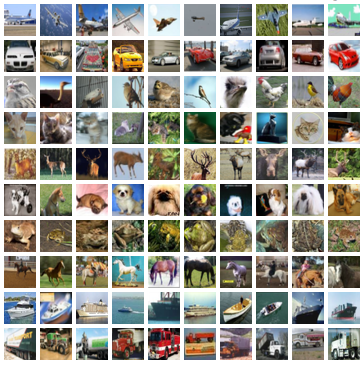
\includegraphics[width=0.5\textwidth]{cifar10}
\caption{10 случайных изображений из 10 классов датасета CIFAR-10}
\end{figure}

\subsection{Фреймворк Caffe}
Свёрточные нейронные сети обучались с помощью фреймворка для глубокого обучения Caffe \cite{jia2014caffe}.
Изначально фреймворк разрабатывался командой BVLC (Berkeley Vision and Learning Center), но постепенно перерос в большой 
open-source проект.\footnote{\url{https://github.com/BVLC/caffe}} На данный момент вклад в развитие Caffe внесли почти 200 
разработчиков и более 10\,000 человек оценили проект на Github.

Данный фреймворк был выбран для решения задачи по нескольким причинам:
\begin{enumerate}
    \item Простота определения моделей и методов оптимизации. Архитектуры нейронных сетей
    (Caffe поддерживает топологии сетей в форме любых ациклических графов) и алгоритмы оптимизации удобно и 
    эффективно определяются в специальных конфигурационных файлах типа Google Protocol 
    Buffers\footnote{\url{https://developers.google.com/protocol-buffers/}}. 
    \item Модульность. Caffe позволяет легко изменять архитектуру сети под новые форматы входных данных. Кроме того, в наличии 
    имеется много слоёв и функций потерь.
    \item Скорость вычислений и эффективное использование ресурсов. Caffe заранее выделяет ровно столько памяти сколько нужно для 
    нейронной сети. Операций линейной алгебры такие как умножение, сложение и свёртка выполняются на CPU с помощью BLAS (Basic 
    Linear Algebra Subroutines). На GPU за эти операции отвечают библиотеки cuBLAS и cuDNN 
    \cite{DBLP:journals/corr/ChetlurWVCTCS14}
    \item CLI (command line interface) и интерфейсы для Python и Matlab.
\end{enumerate}

Caffe написан на языках C++, Cuda, Python. Для хранения датасетов используются эффективные базы данных 
LMDB\footnote{\url{http://symas.com/mdb/}} и LevelDB\footnote{\url{https://github.com/google/leveldb}}. Обучение нейронных сетей 
может выполняться как на CPU, так и на нескольких GPU одновременно. Фреймворк доступен для Linux, Windows и OS X.

\subsection{Предварительная обработка данных}
Необработанные изображения содержат излишнюю информацию, так как смежные пиксели имеют высокую корреляцию. Поэтому прежде чем 
подавать изображения на вход нейронной сети, они были обработаны в два этапа. В начале была произведена глобальная нормализация контраста
(global contrast normalization) изображения:
\[ \widehat{X} = \cfrac{X - \overline{X}}{\sigma},\]
где $X$ --- исходное изображение, $\overline{X}$ --- среднее значение, $\sigma$ --- стандартное отклонение.

Затем изображения были линейно трансформированы с помощью алгоритма ZCA whitening \cite{learningmultiple}.
Цель данного алгоритма сделать так, чтобы входные изображения слабо коррелировали друг с другом.

Алгоритм ZCA whitening:
\begin{lstlisting}[language=Python, frame=TB]
cov = np.dot(X.T, X) / X.shape[0] #%* Вычисляем ковариационную матрицу *)
U,S,V = np.linalg.svd(cov) #%* Находим сигнулярное разложение ковариацонной матрицы *)
Xrot = np.dot(X, U) #%* Поворачиваем входные данные *)
Xwhite = Xrot / np.sqrt(S + %*$\alpha$*)) #%* Делим на собственные числа *)
\end{lstlisting}
\vspace*{-1.4cm}
\begin{figure}[h]
    \centering
    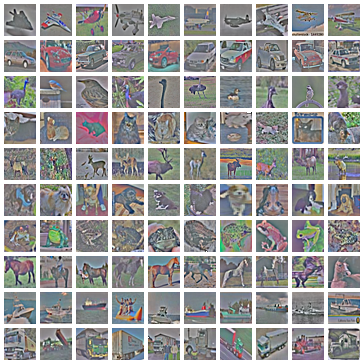
\includegraphics[width=0.5\textwidth]{cifar10zca}
    \caption{Изображения после применения ZCA whitening с параметром $\alpha=0,1$}
\end{figure}
Предобработка с помощью ZCA whitening уменьшила ошибку в среднем на $1,5\%$. Кроме того, каждое изображение было
увеличено до 40$\times$40 пикселей, для того чтобы в процессе обучения вырезать из 
изображения случайный патч размером 32$\times$32. Такой приём позволяет снизить эффект переобучения модели и повысить конечную 
точность распознавания.

\subsection{Обучение нейронных сетей}
Во время исследования были проверены различные гипотезы, архитектуры и эвристики так или иначе влияющие на конечные точности 
моделей. В результате различных экспериментов были отобраны семь нейронных сетей, показавшие наилучший результат.
Топологии этих сетей отражены в таблице~\ref{models-table}, графики обучения на рисунке \ref{fig:train_all}.
Инициализация весов во всех моделях проводилась с помощью layer-sequential unit-variance (LSUV) \cite{DBLP:journals/corr/MishkinM15}.
Данный метод сначала проводит преинициализацию весов ортонормированными матрицами \cite{DBLP:journals/corr/SaxeMG13},
затем, для каждого слоя настраивает параметры таким образом, чтобы дисперсия выходов была единичной.
Далее будут описаны каждая из отобранных моделей, их свойства и особенности обучения.

\subsubsection{Модель I}
Модель I имеет самую низкую ошибку в предсказаниях среди всех обученных моделей ($6,6$\%). СНН состоит из 18 обучающихся слоёв.
Всего в нейронной сети $\approx$\,2,7 млн. параметров.

Maxout в качестве функции активации является её отличительной особенностью.
На рисунке~\ref{fig:model_I_maxout_example} показано как maxout соединён с выходами свёрточных слоёв. На
рисунке~\ref{fig:model_I_maxout_ip_example} можно видеть соединение выходов полносвязного слоя и активации.

\begin{figure}[H]
\centering
\begin{minipage}{.5\textwidth}
  \centering
  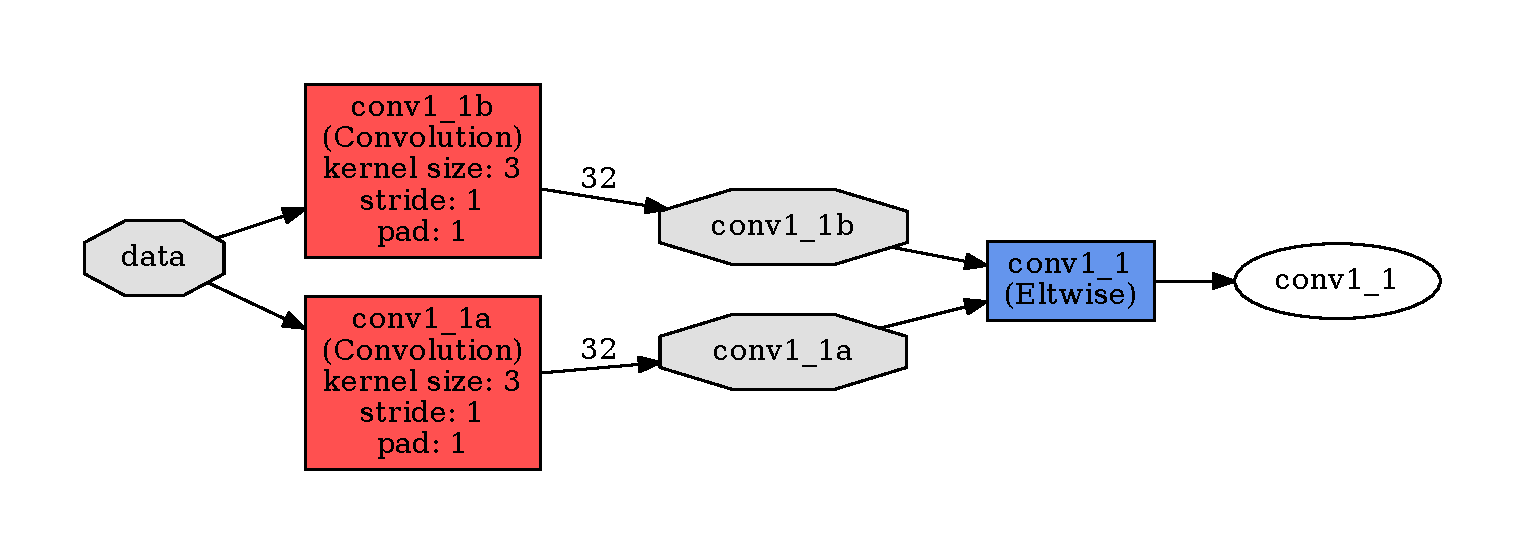
\includegraphics[width=\textwidth]{model_I_maxout_example}
  \captionof{figure}{Соединение maxout'а со\\
                     свёрточными слоями}
  \label{fig:model_I_maxout_example}
\end{minipage}%
\begin{minipage}{.5\textwidth}
  \centering
  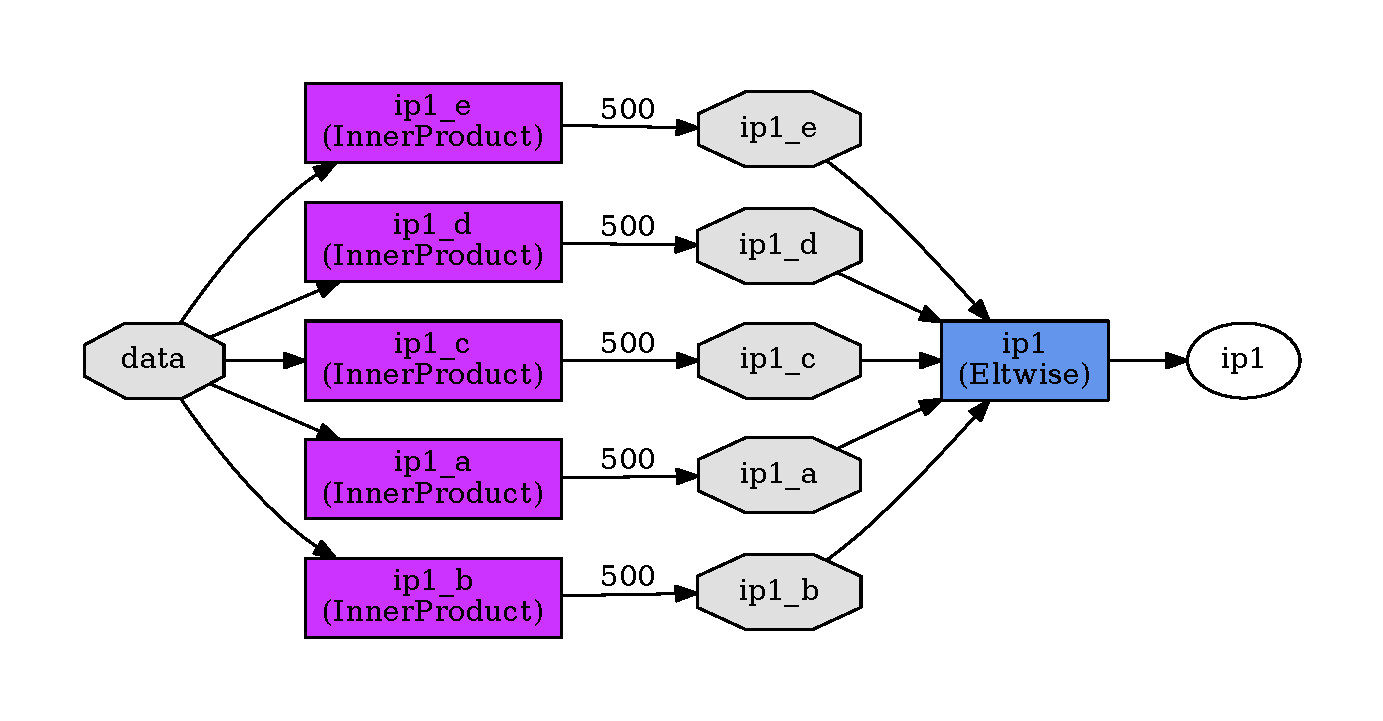
\includegraphics[width=\textwidth]{model_I_maxout_ip_example}
  \captionof{figure}{Соединение maxout'а с\\
                     полносвязными слоями}
  \label{fig:model_I_maxout_ip_example}
  \vspace*{1.4cm}
\end{minipage}
\vspace*{-1.4cm}
\end{figure}

Нейронная сеть обучалась 90\,000 итераций методом стохастического градиентного спуска,
с начальным learning rate (lr) 0,01 и моментом 0.9. Кроме того, использовалась L2 регуляризация с коэффициентом 0,0005.
В процессе обучения, начиная с 40\,000 итерации, lr уменьшался в десять раз каждые 20\,000 итераций.
Таким образом, к концу обучения lr достиг значения $10^{-5}$. Mini batch состоял из 256 изображений.

\begin{figure}[H]
    \centering
    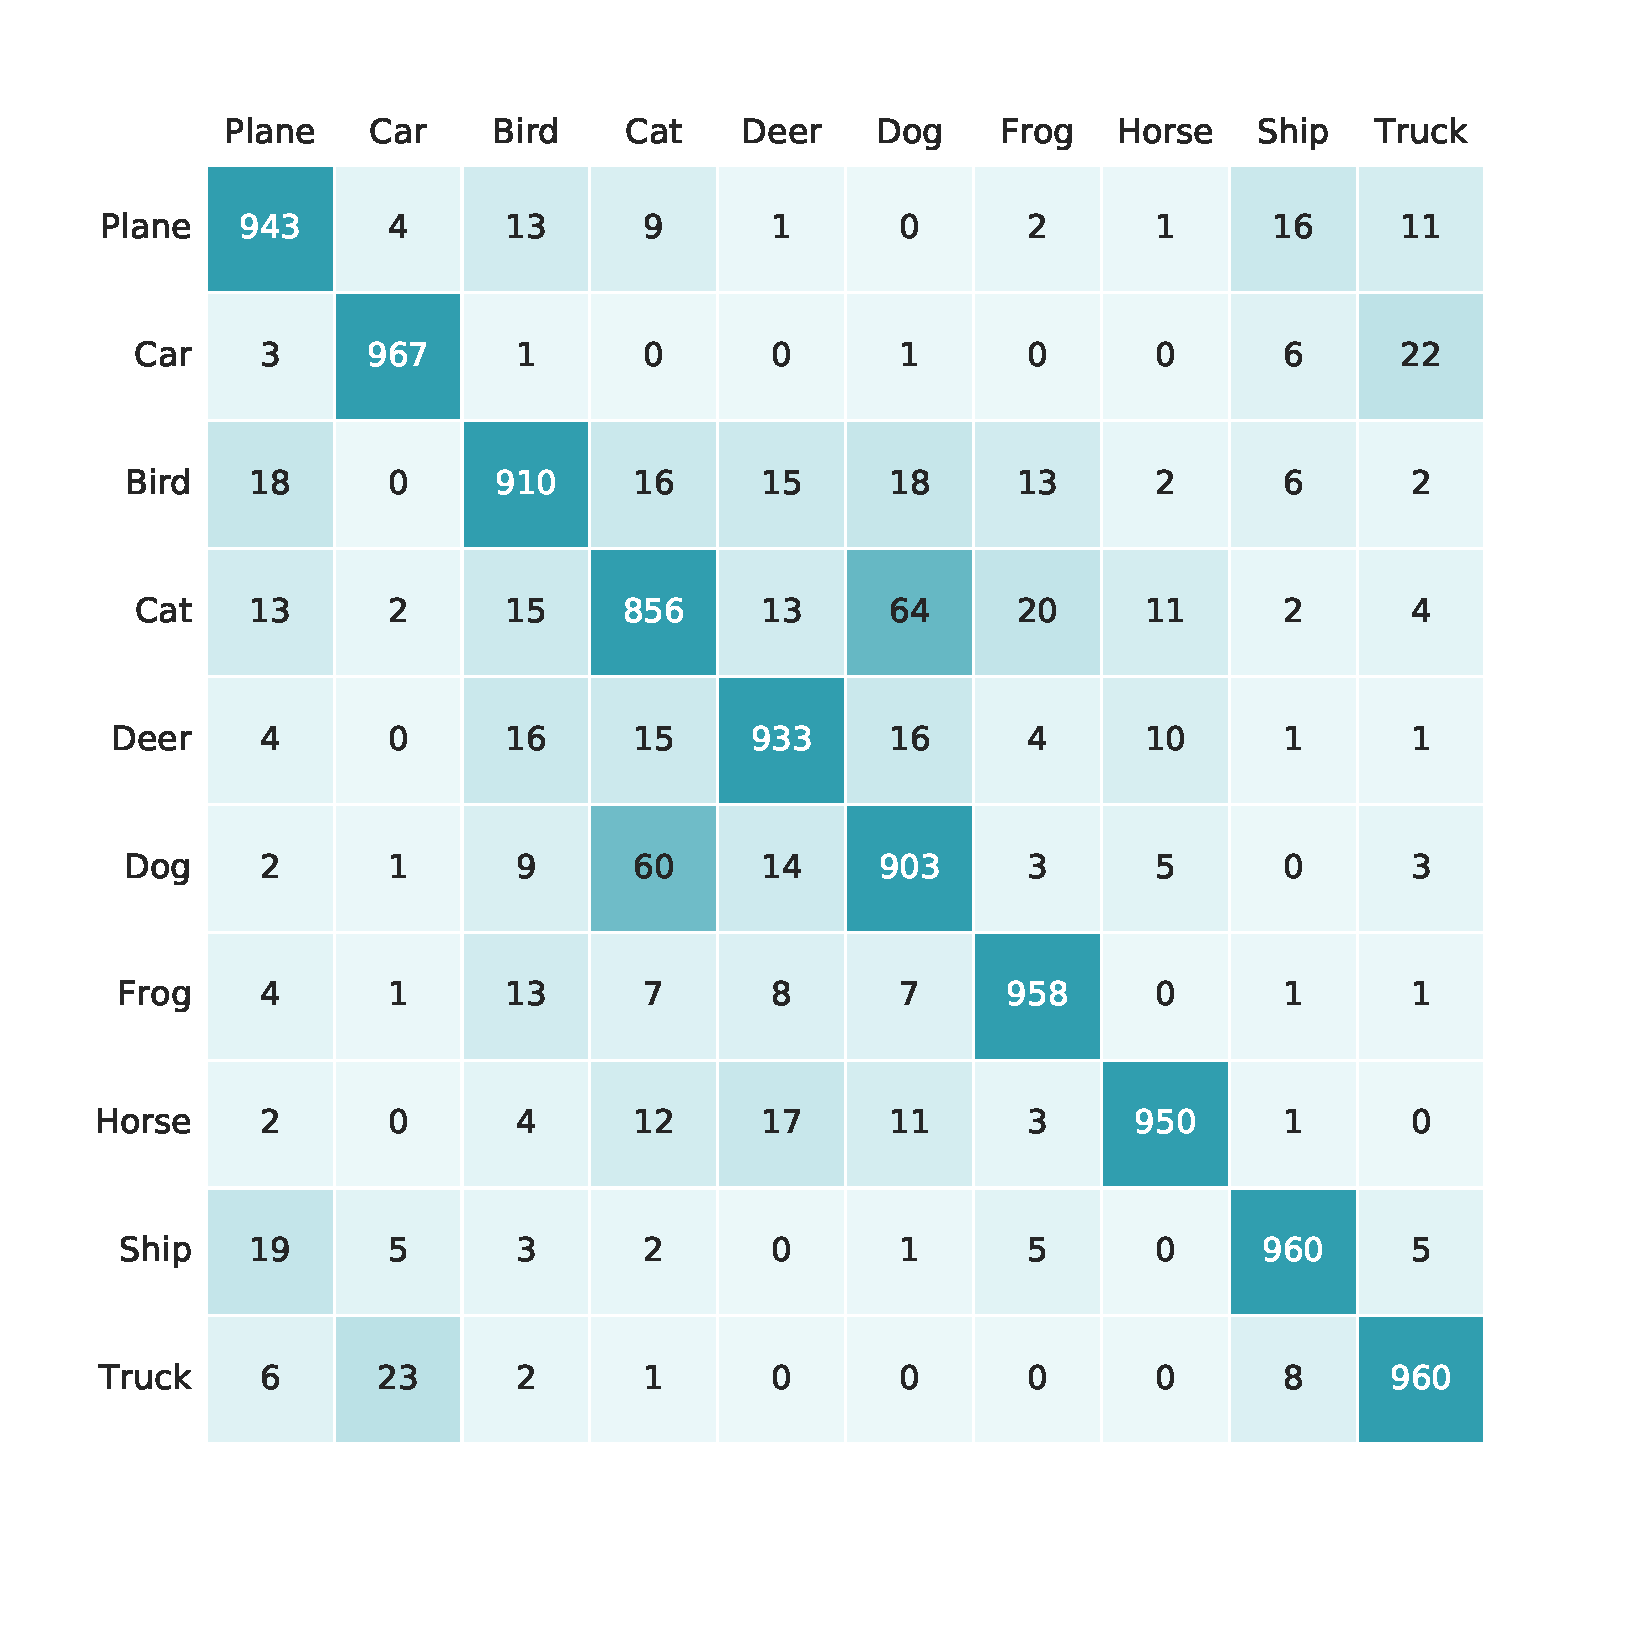
\includegraphics[width=0.5\textwidth]{confusion_matrix_model_I}
    \vspace*{-0.5cm}
    \caption{Матрица ответов модели I}
    \label{fig:confusion_matrix_model_I}
\end{figure}

\subsubsection{Модели II и III}
Модель II имеет в 4,5 раза меньше параметров, в сравнении с моделью I. Их число составляет $\approx$\,600\,000.
Данная нейронная сеть имеет классическую архитектуру --- чередование свёрточных и pooling слоёв, в качестве
функции активации используется Leaky ReLU\footnote{$f(x) = \max(x, \alpha x)$} с параметром $\alpha = 0,01$.

Сеть обучалась в течении 30\,000 итераций. Функционал ошибки оптимизировался алгоритмом Нестерова.
Результат модели II оказался ниже на тестовом множестве, в сравнении с моделью I (89,4\% против 93,4\%).
Данный результат объясняется недообучением, что является следствием недостаточного числа параметров нейронной сети.
С другой стороны, за счёт уменьшения числа весов в модели, удалось снизить время обучения в 10 раз (с десяти часов до одного).

Модель III является попыткой исправить главный недостаток модели II за счёт увеличения числа параметров.
В связи с чем, число фильтров каждого свёрточного слоя было увеличено в два раза, что позволило снизить ошибку на 1,6\%.

\begin{figure}[H]
\centering
\begin{minipage}{.5\textwidth}
  \centering
  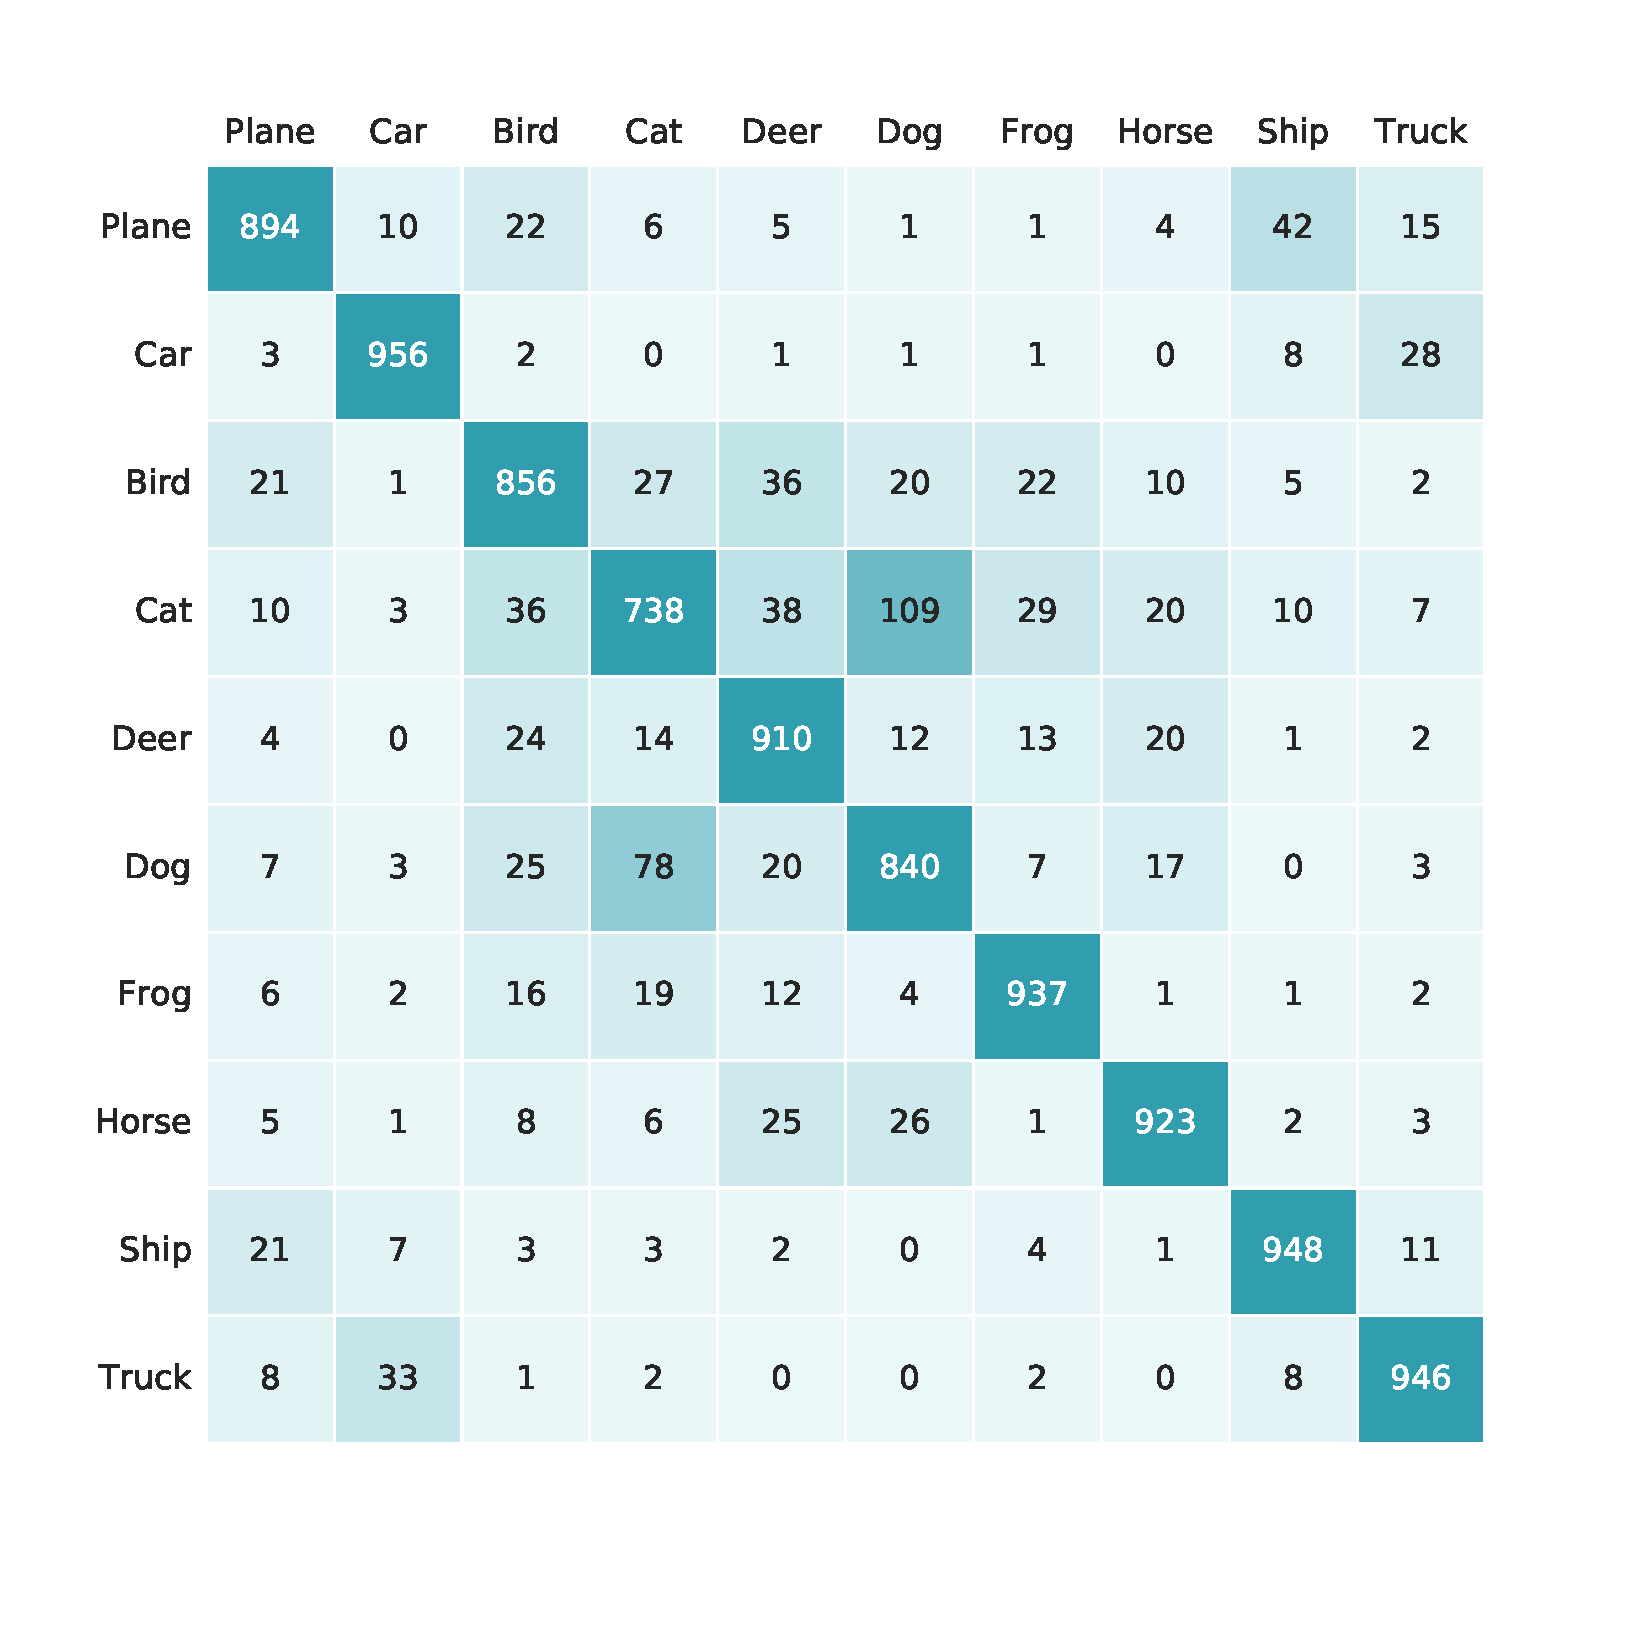
\includegraphics[width=\textwidth]{confusion_matrix_model_II}
  \captionof{figure}{Матрица ответов\\модели II}
\end{minipage}%
\begin{minipage}{.5\textwidth}
  \centering
  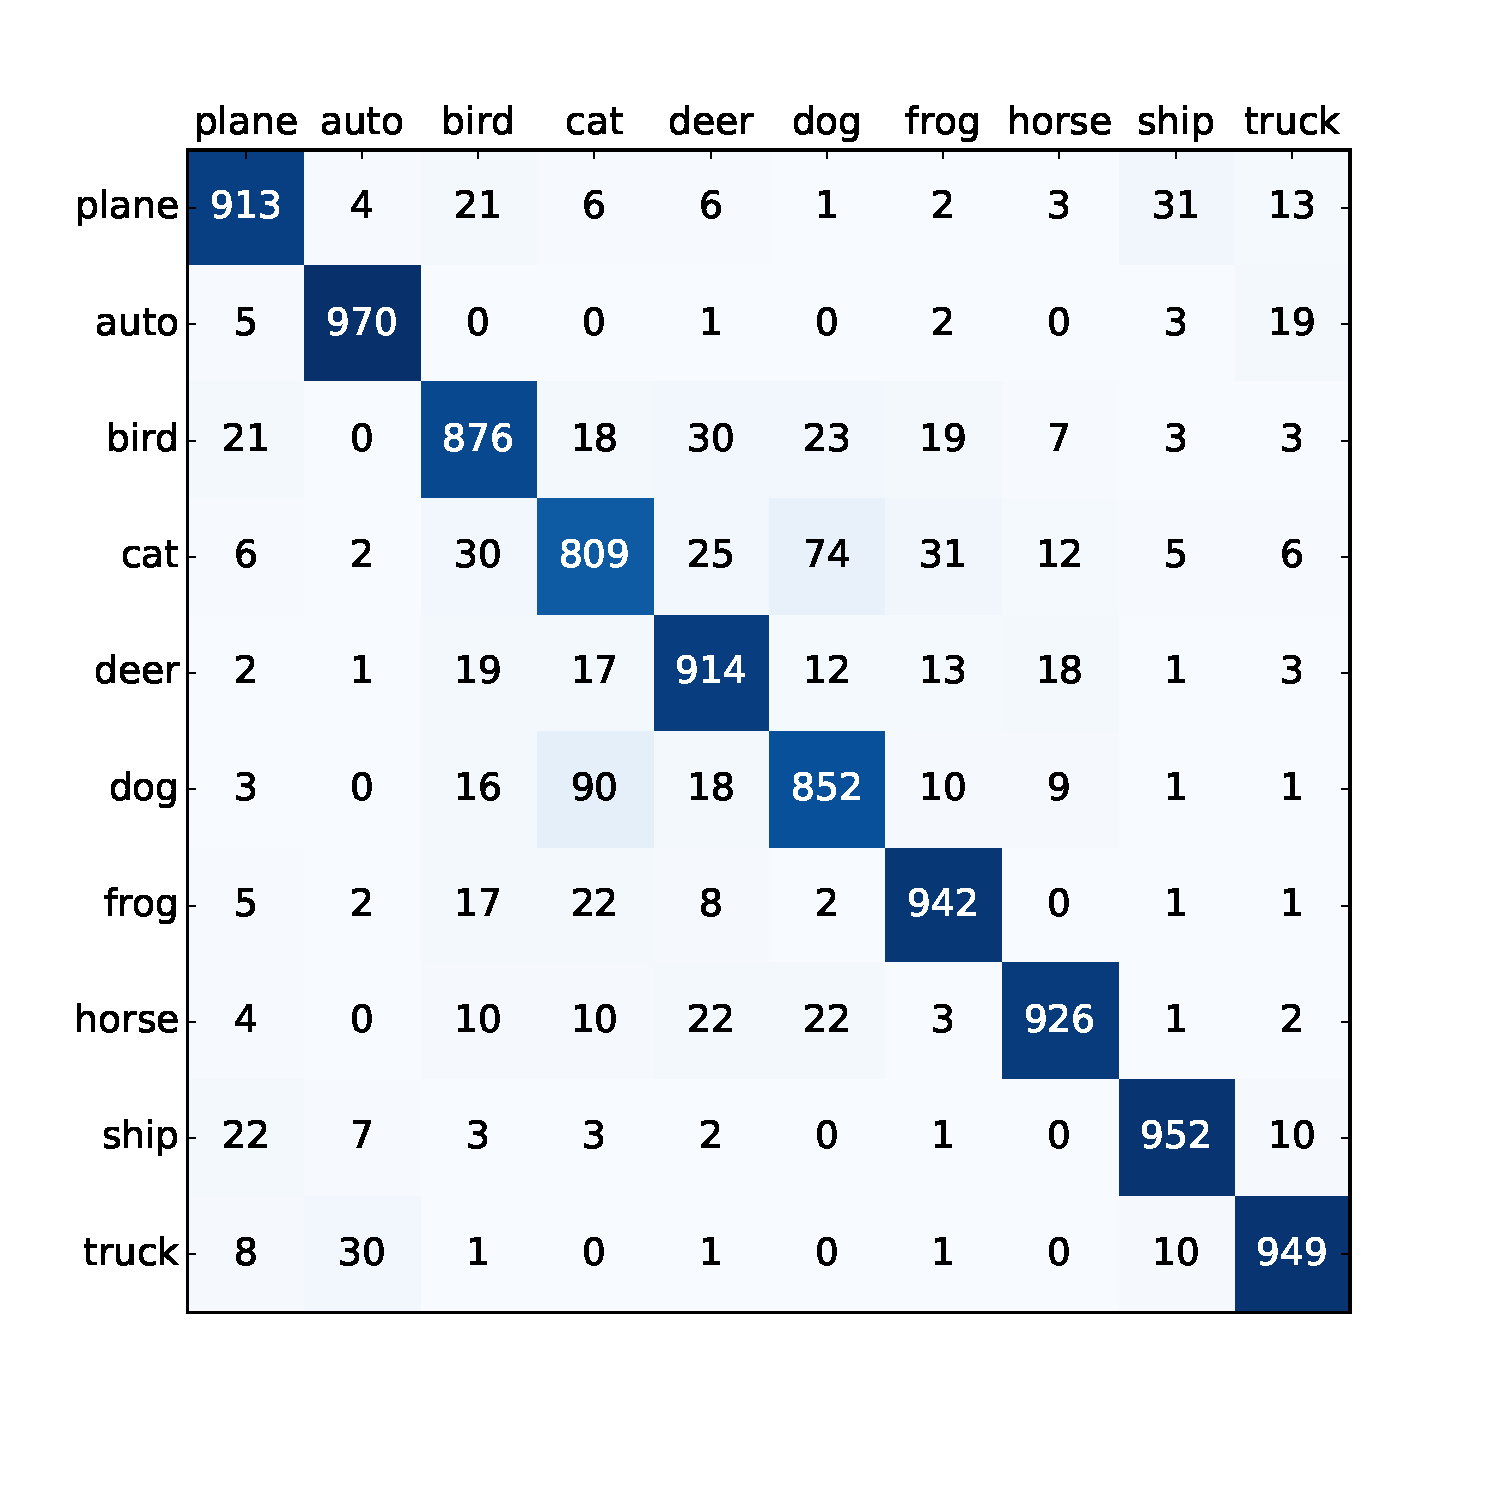
\includegraphics[width=\textwidth]{confusion_matrix_model_III}
  \captionof{figure}{Матрица ответов\\модели III}
\end{minipage}
\end{figure}

\subsubsection{Модели IV и V}
На моделях IV и V проверялась гипотеза, основная идея которой в том, что pooling слои могут быть заменены
на соответствующие свёрточные слои с увеличенным параметром stride без значительного снижения точности распознавания.
\cite{DBLP:journals/corr/SpringenbergDBR14}. В данных сетях max-pooling~2$\times$2 слои были заменены 
на свёрточные слои со stride равным двум.

Модель IV имеет $\approx$\,6 млн. параметров и 13 слоёв. В качестве функции активации используется ReLU.
После обучения в течении 14 часов и 50\,000 итераций, точность на тестовом множестве достигла 92,1\%, что
подтверждает гипотезу о замене pooling слоёв.

Модель V состоит из 16 слоёв и $\approx$\,7,8 млн свободных параметров. Данная нейронная сеть является попыткой
улучшить точность модели IV за счёт увеличения числа свёрточных слоёв. Однако, дополнительные слоёв привнесли
дополнительно $\approx$\,1.8 млн. параметров, что привело к переобучению и снижении конечной точности на 1,2\%.
Модель V обучалась в течении 50\,000 итераций, что заняло 19 часов.

\subsubsection{Модель VI}
Модель VI состоит из 18 слоёв и $\approx$\,4,2 млн. параметров. Данная модель использует слои batch normalization, 
которые преобразовывают активаций свёрточных и полносвязных слоев таким образом, что их среднее равно нулю, а
дисперсия единице (значения вычисляются на всём mini batch). Авторы batch normalization \cite{DBLP:journals/corr/IoffeS15}
утверждают, что данный приём позволяет использовать высокий learning rate и приводит к более быстрой сходимости.
Модель VI достигла точности в 92,0\% за 25\,0000 итераций, а общее время затраченное на обучение (40\,000 итераций)
заняло 6 часов.
\begin{figure}[H]
    \centering
    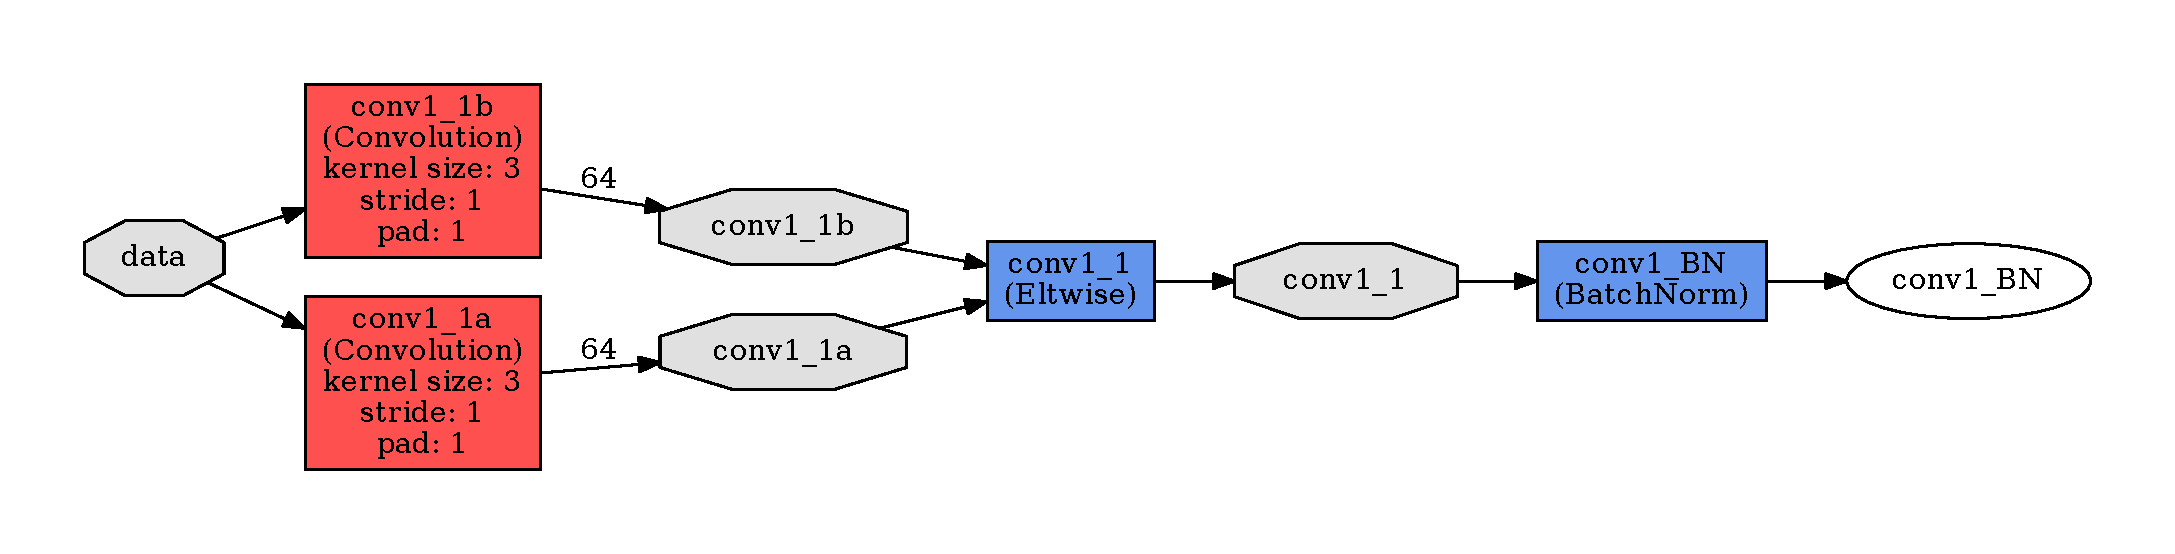
\includegraphics[width=0.9\textwidth]{batchnrm_net_VI}
    \caption{Batch normalization слой в модели~VI}
    \label{fig:model_VI_bnrm}
\end{figure}

\begin{figure}[H]
    \centering
    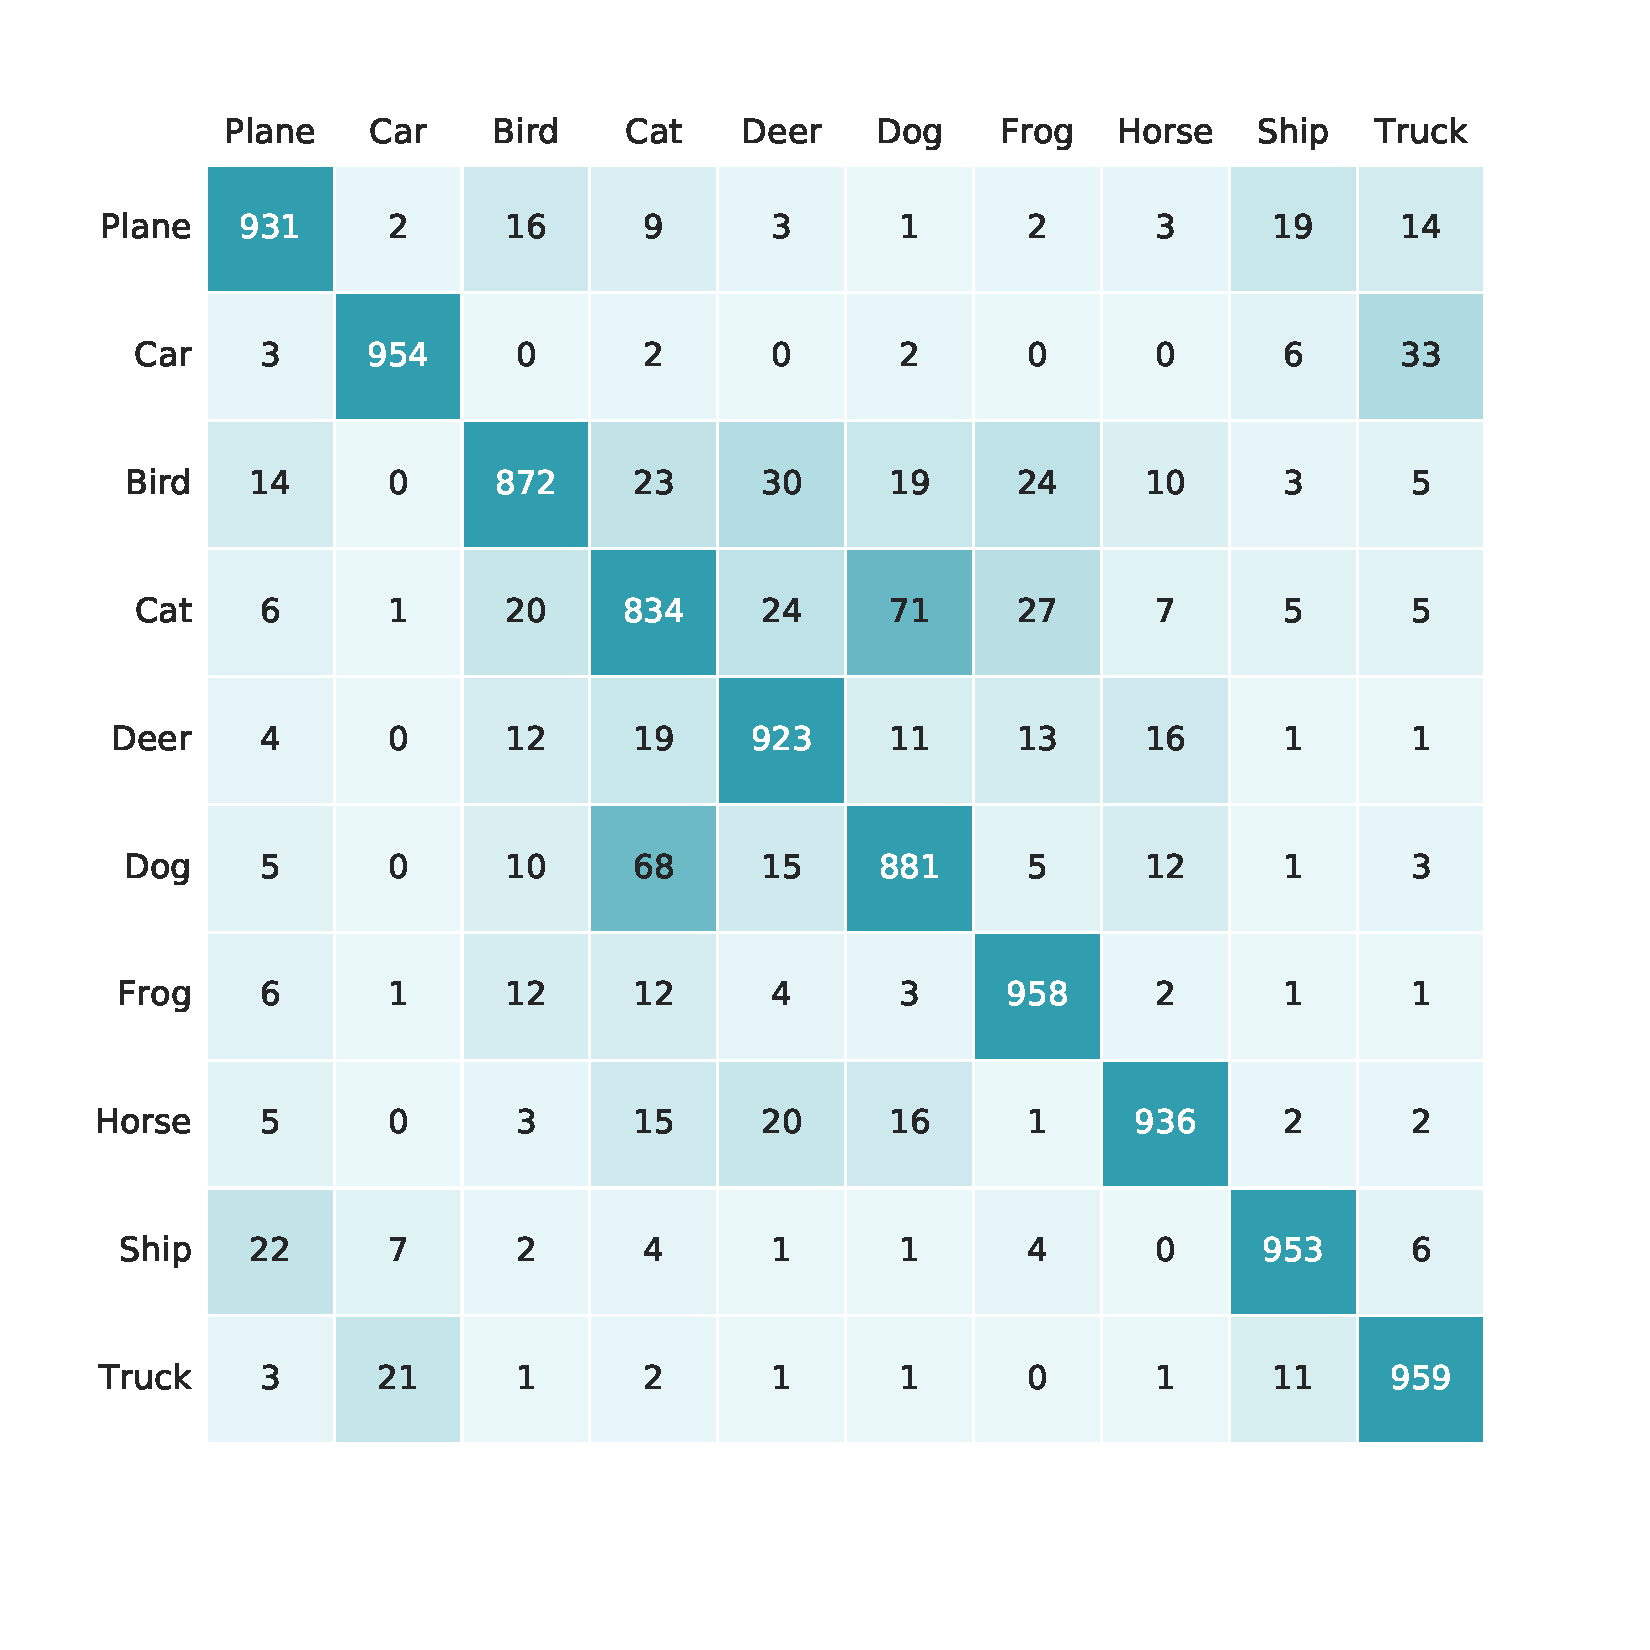
\includegraphics[width=0.5\textwidth]{confusion_matrix_model_VI}
    \vspace*{-0.5cm}
    \caption{Матрица ответов модели VI}
    \label{fig:confusion_matrix_model_VI}
\end{figure}

\subsubsection{Модель VII}
Модель VII идентична модели I, за исключением количества свёрточных слоёв соединённых с maxout активацией. В данной модели их пять
(Рис. \ref{fig:model_VII_maxout}), тогда как модель I имеет только два слоя. Такое изменение в топологии сети не привело к 
увеличению конечной точности модели, более того, ошибка увеличилась на 0,9\%. Максимальное число итераций достигло 70\,000,
время затраченное на обучение составило 22 часа.
\begin{figure}[H]
    \centering
    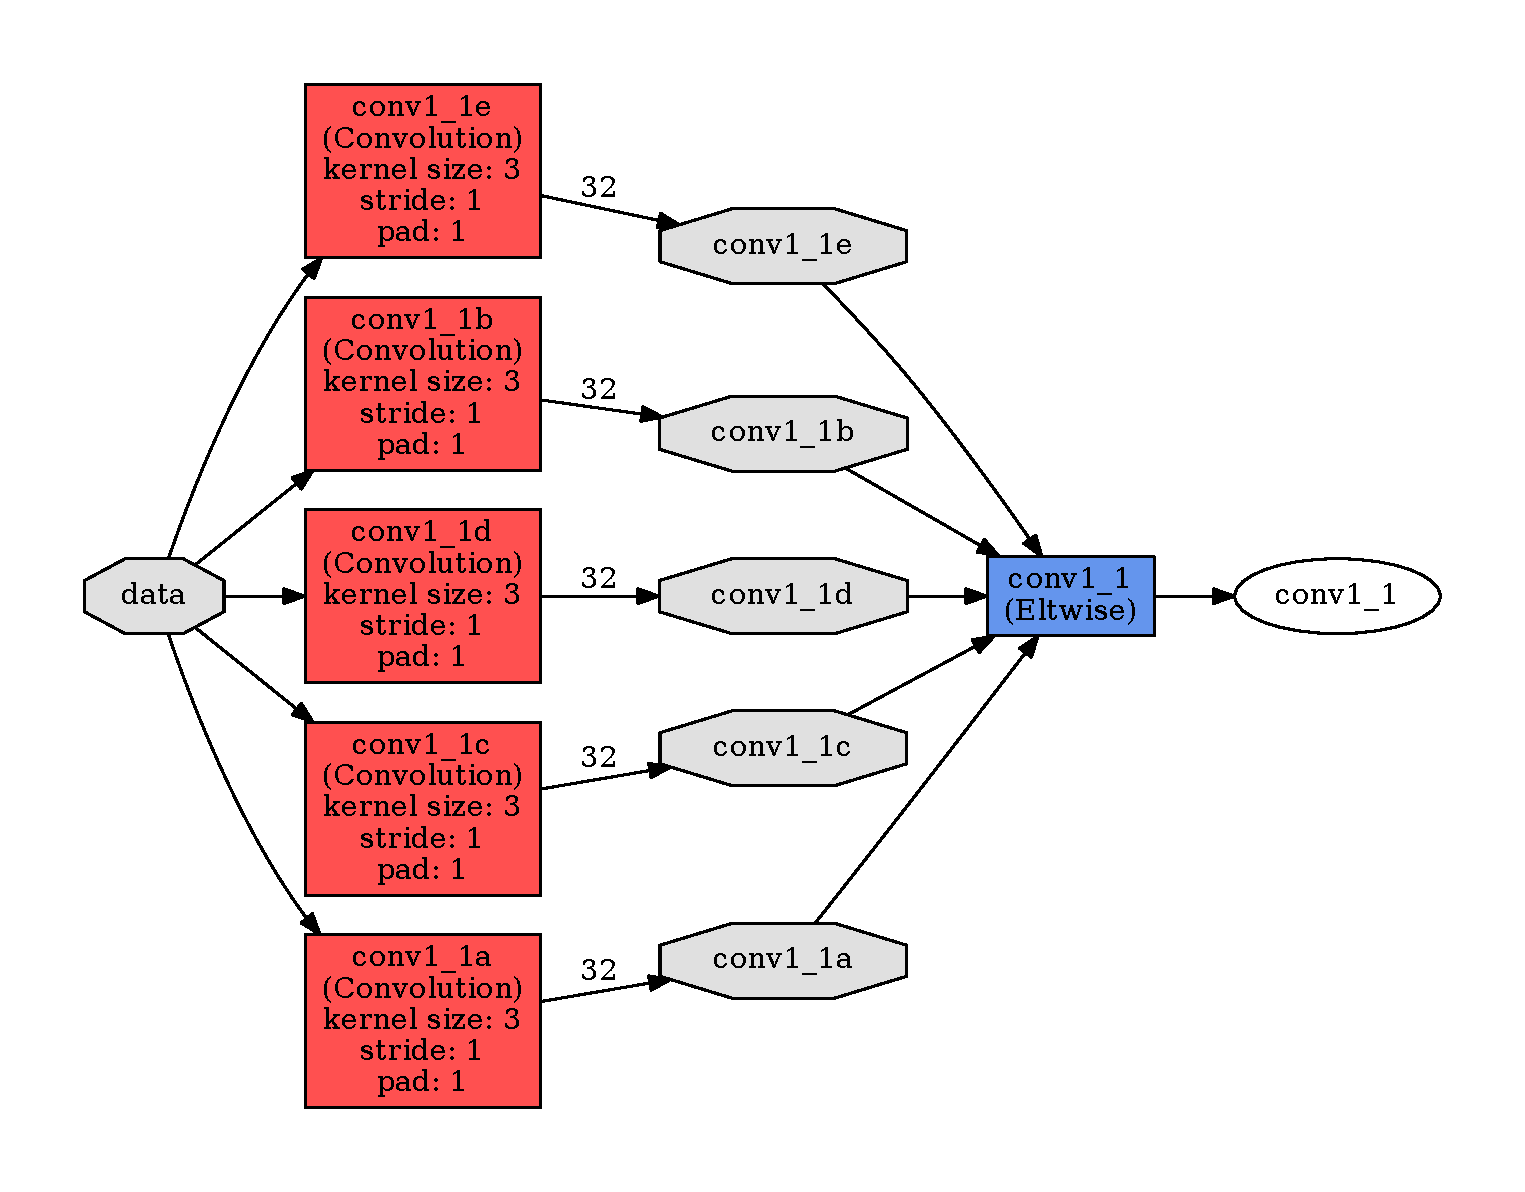
\includegraphics[width=0.5\textwidth]{model_VII_maxout}
    \caption{Соединение maxout активаций в модели~VII}
    \label{fig:model_VII_maxout}
\end{figure}

\begin{figure}[H]
    \centering
    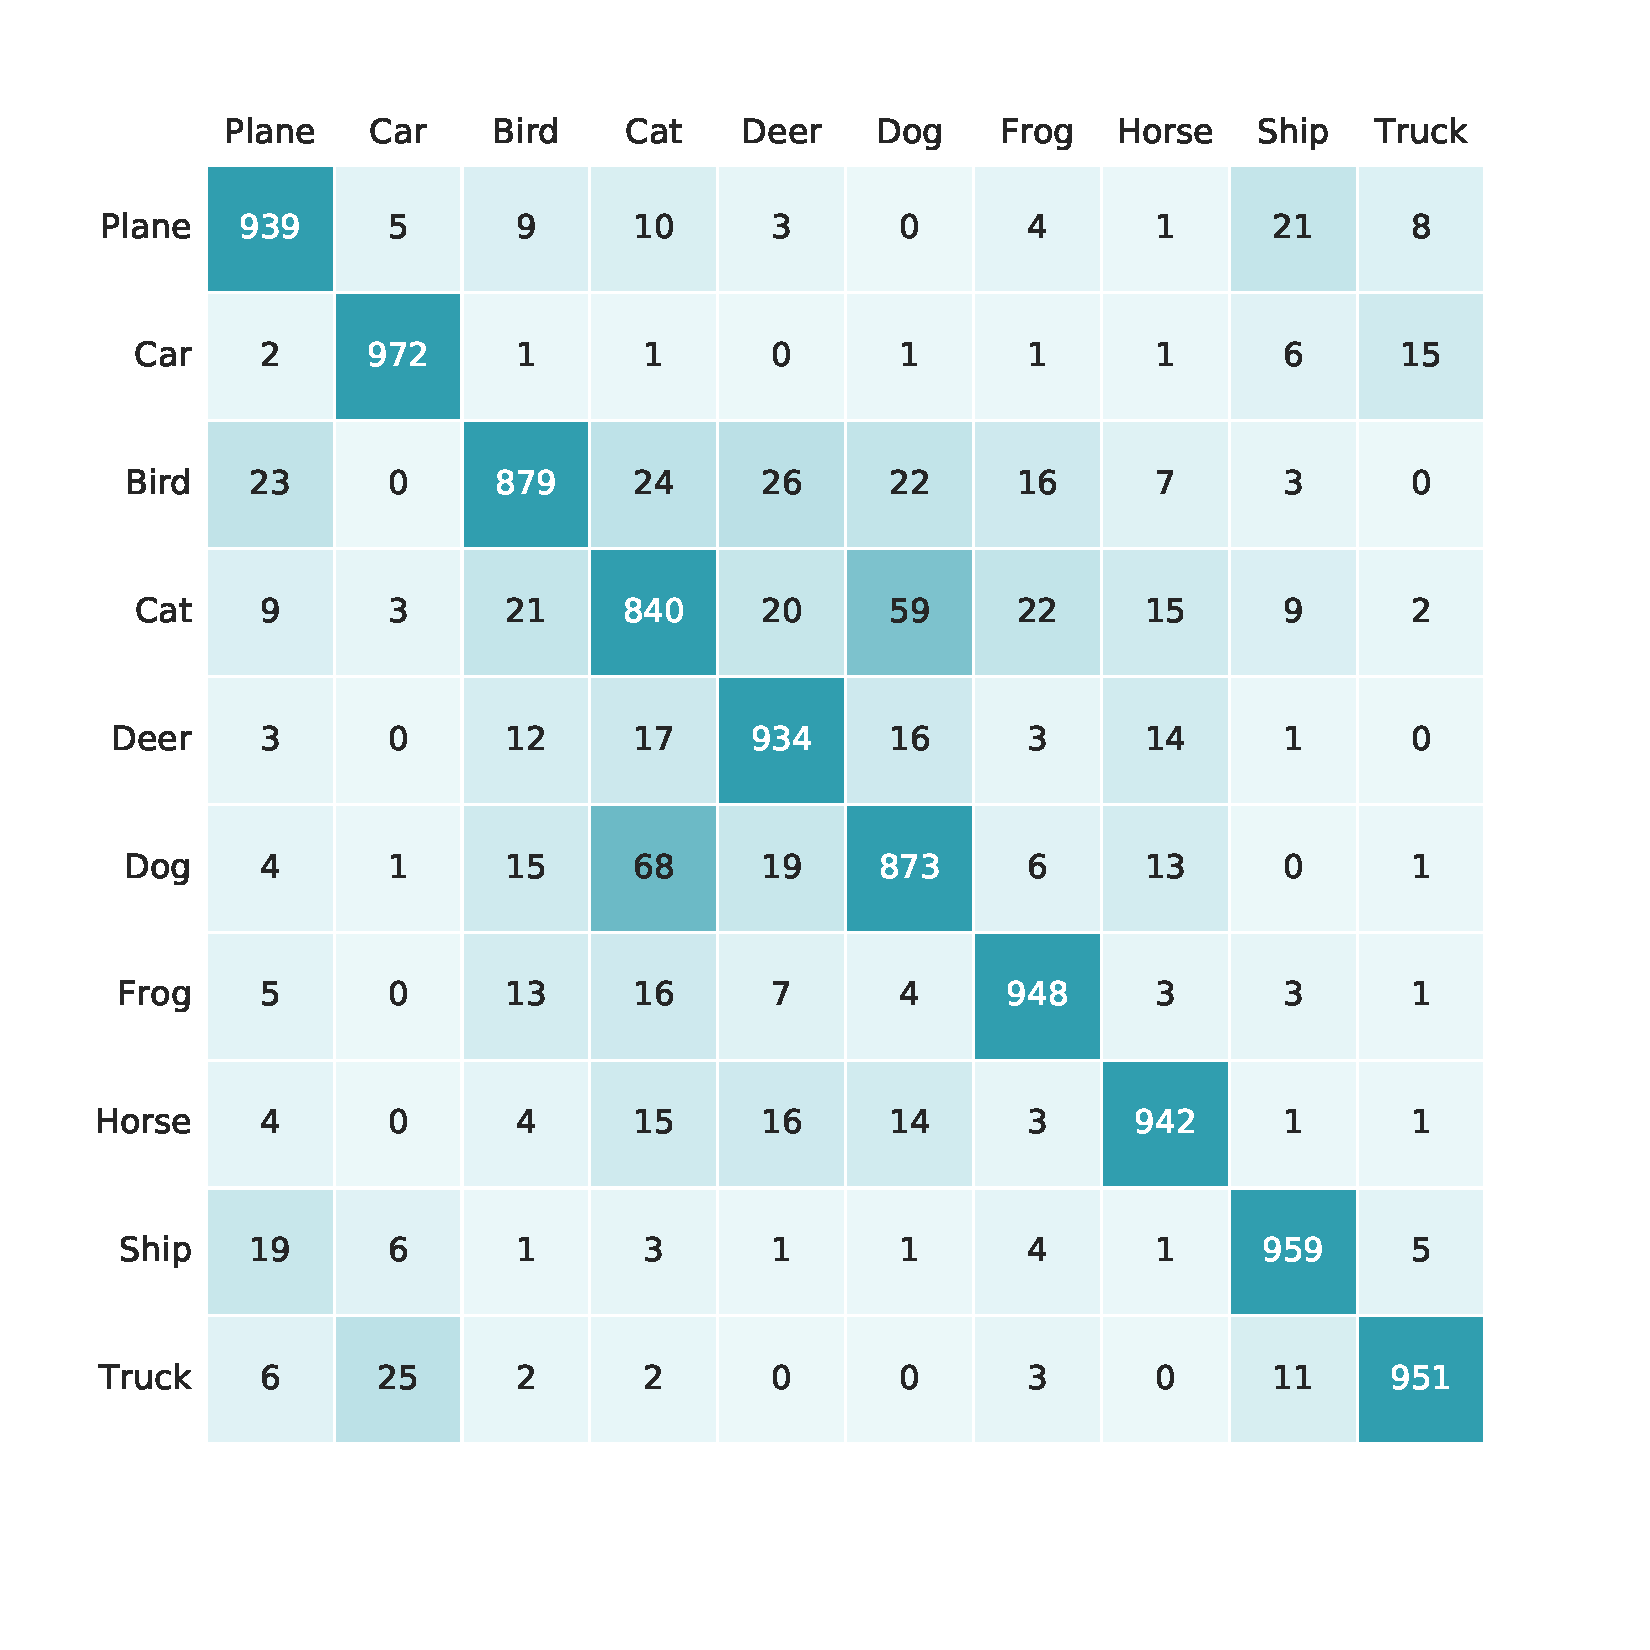
\includegraphics[width=0.5\textwidth]{confusion_matrix_model_VII}
    \vspace*{-0.5cm}
    \caption{Матрица ответов модели VII}
    \label{fig:confusion_matrix_model_VII}
\end{figure}

\subsection{Объединение нейронных сетей в ансамбль}
Объединение нескольких моделей в ансамбль является мощным приёмом при решении различных задач машинного обучения.
Применение подобной техники было выбрано по причине наличия различных свёрточных нейронных сетей, предсказания которых
не очень сильно коррелируют между собой. В данном исследовании модели объединялись с помощью <<стэкинга>> (stacking)
\cite{Wolpert92stackedgeneralization}, идея которого заключается в построении алгоритма, который делает финальные 
предсказания, основываясь на ответах других моделей (в данном случае на ответах нейронных сетей). Такой подход зачастую
работает лучше любой из одиночных моделей.

Для построения конечного ансамбля были протестированы различные алгоритмы классификации, такие как случайный лес, 
метод k ближайших соседей, персептрон и SVM. Наилучшая точность была достигнута с помощью SVM (94,15\%) с радиально-базисной
функцией ядра (RBF kernel function). Конечная схема классификатора отражена на рисунке \ref{fig:ansamble}.

\begin{figure}[H]
    \centering
    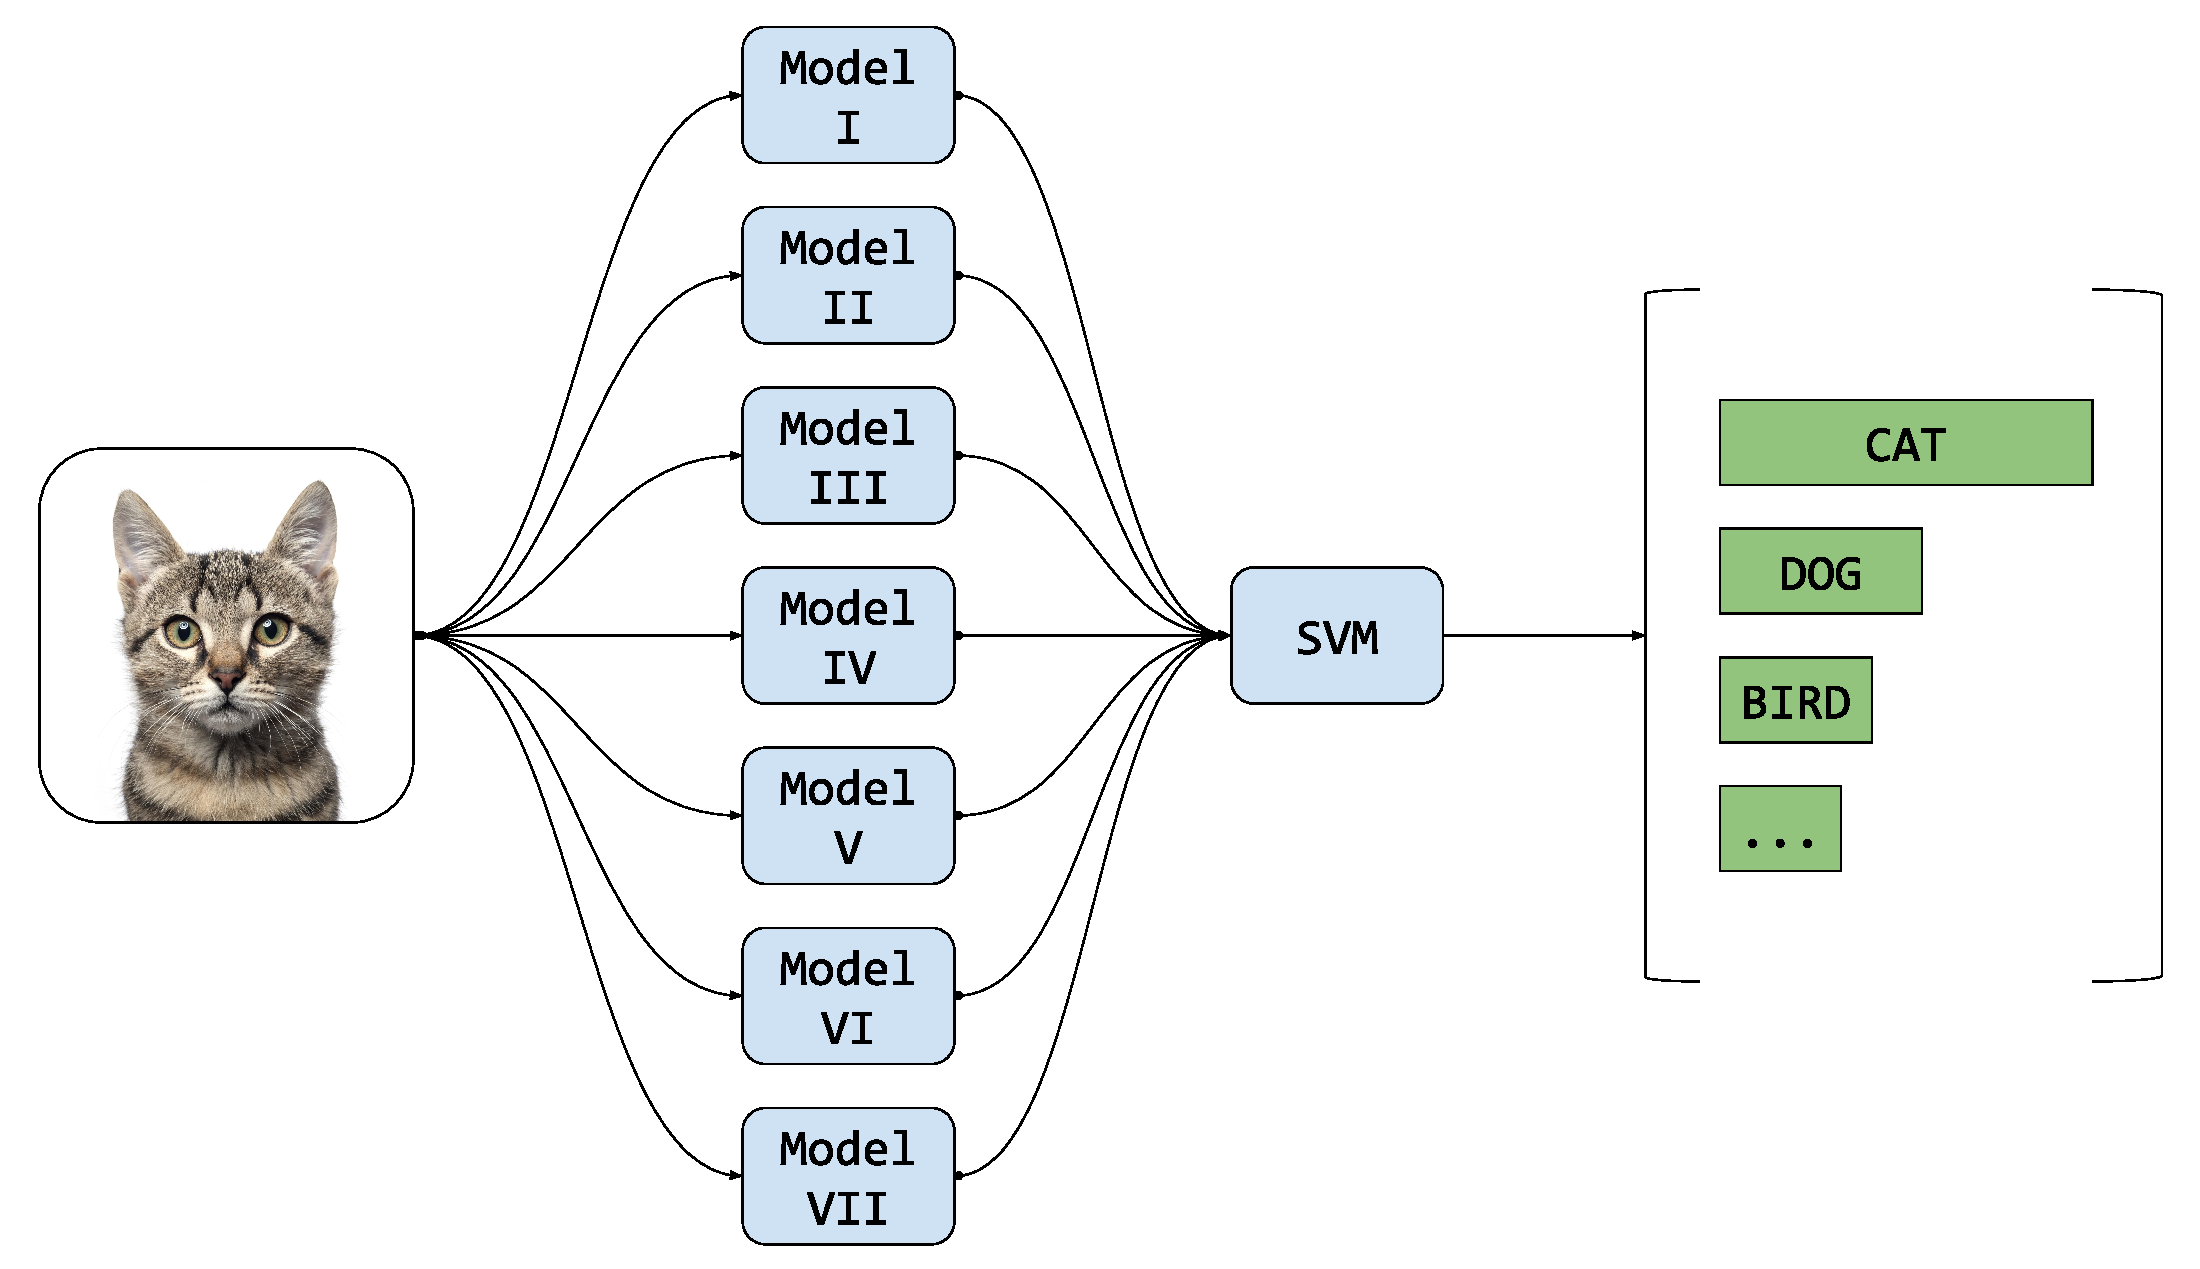
\includegraphics[width=0.6\textwidth]{ensamble}
    \caption{Схема конечного ансамбля моделей}
    \label{fig:ansamble}
\end{figure}

\begin{figure}[H]
    \centering
    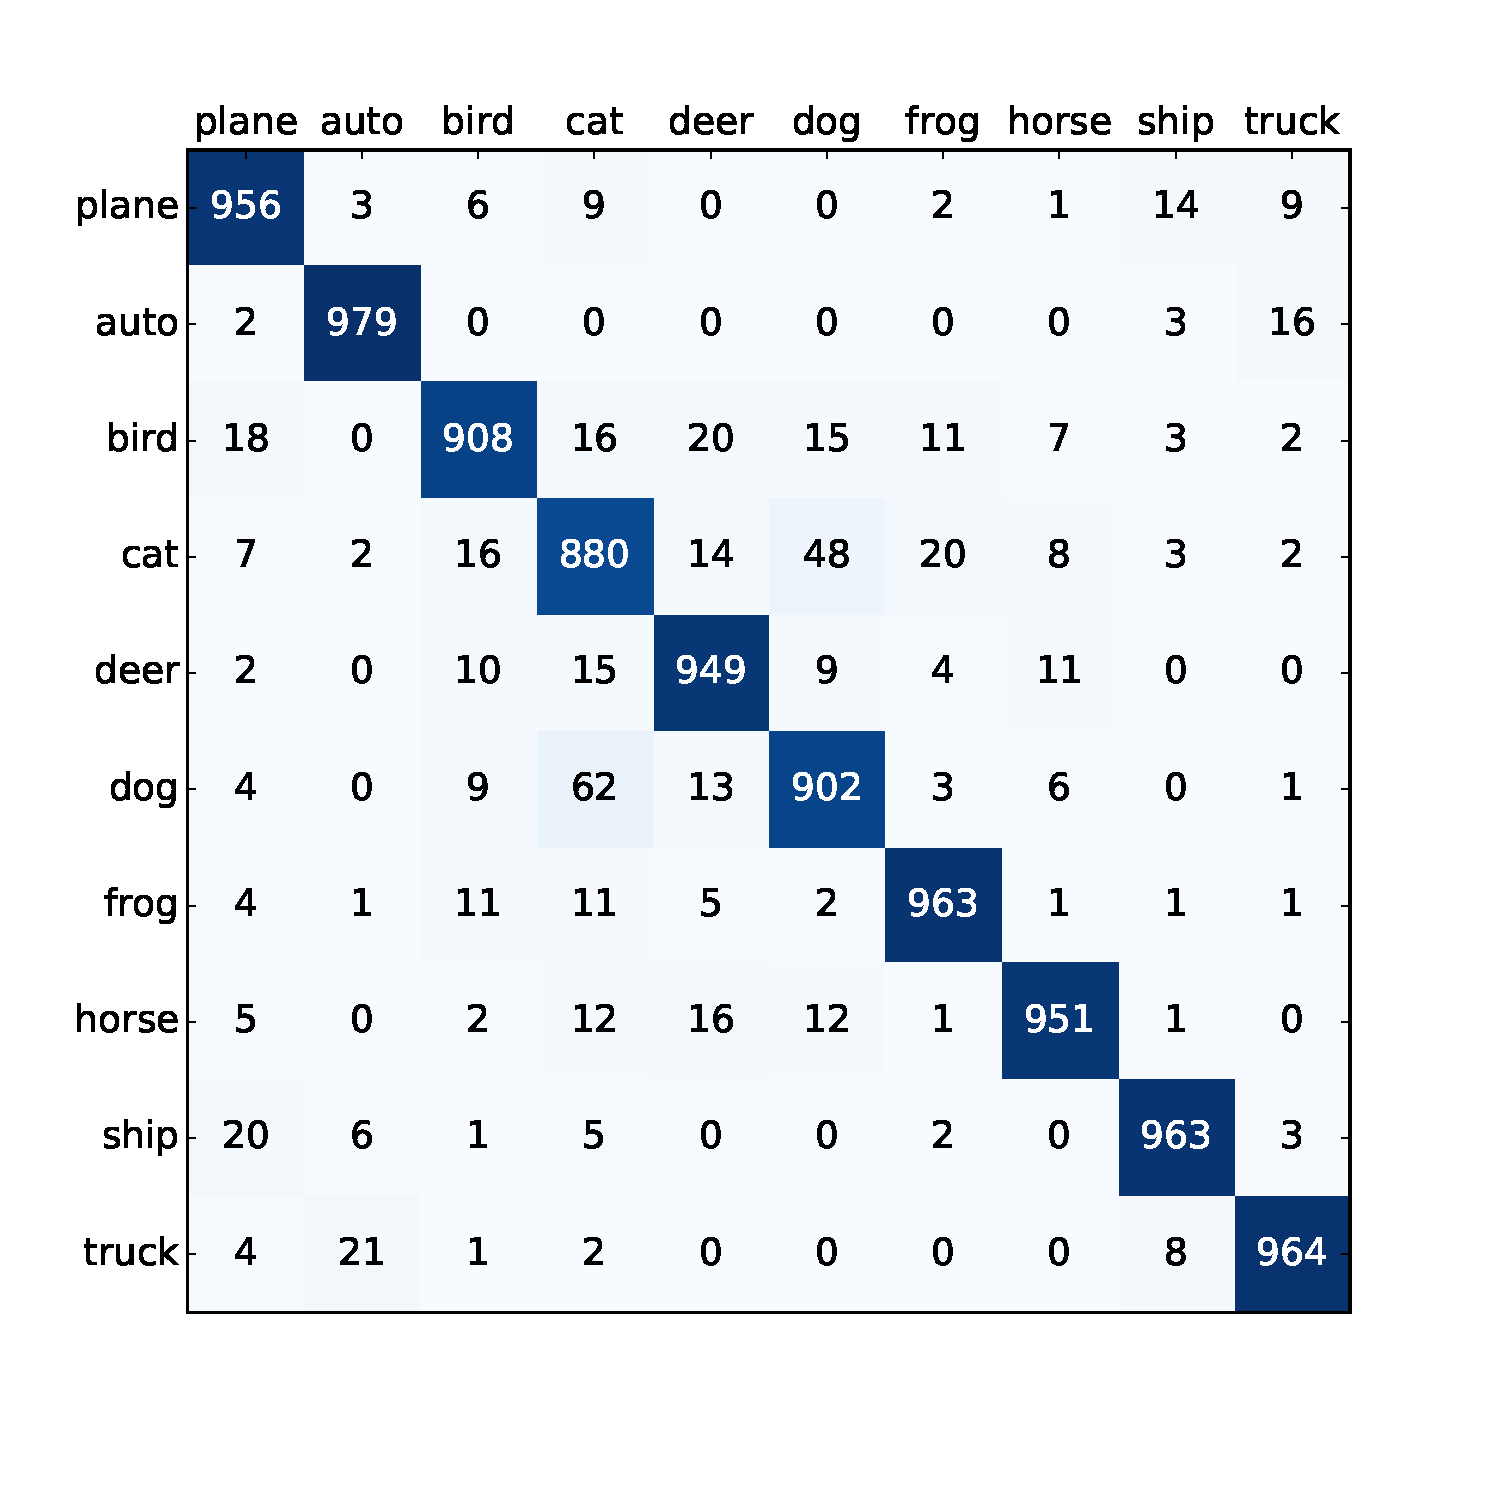
\includegraphics[width=0.5\textwidth]{ensamble_confusion_matrix}
    \vspace*{-0.5cm}
    \caption{Матрица ответов ансамбля моделей}
    \label{fig:ensamble_confusion_matrix}
\end{figure}